\documentclass[10pt]{beamer}

\usepackage[english]{babel}
\usepackage[utf8]{inputenc}
\usepackage{amsmath,amssymb,amsthm,latexsym}
\usepackage{mathrsfs}
\usepackage[all]{xypic}
\usepackage{tikz}
\usetikzlibrary{arrows,shapes,automata}
\usepackage{eurosym}
\usepackage{listings}
\usepackage{textcomp}

\newcommand{\cat}[1]{\mathscr{#1}}
\newcommand{\lcat}[1]{\mathbf{#1}}
\renewcommand{\L}{\cat{L}}
\newcommand{\comp}{\circ}
\newcommand{\size}[1]{\lVert#1\rVert}
\newcommand{\sizein}[1]{\size{#1}^\mathrm{in}}
\newcommand{\sizeout}[1]{\size{#1}_\mathrm{out}}
\DeclareMathOperator{\ob}{ob}
\DeclareMathOperator{\Hom}{Hom}
\DeclareMathOperator{\id}{id}
\DeclareMathOperator{\Id}{Id}
\newcommand{\N}{\mathbb{N}}
\newcommand{\Z}{\mathbb{Z}}
\newcommand{\C}{\mathbb{C}}
\newcommand{\R}{\mathbb{R}}
\newcommand{\K}{\mathbb{K}}
\newcommand{\LK}{\mathbb{L}}
\newcommand{\ra}{\rightarrow}
\newcommand{\la}{\leftarrow}
\DeclareMathOperator{\Time}{t}
\DeclareMathOperator{\Space}{s}
\DeclareMathOperator{\coTime}{co-t}
\DeclareMathOperator{\coSpace}{co-s}
\DeclareMathOperator{\Par}{Par}
\DeclareMathOperator{\Tr}{Tr}
\DeclareMathOperator{\rev}{rev}
\newcommand{\computes}{\vdash}
\renewcommand{\u}{\underline}
\renewcommand{\o}{\overline}
\newcommand{\tALpy}{\texttt{transalpyne}}

\lstset{
  language=haskell,
  upquote=true,
  basicstyle=\ttfamily\small,          % print whole listing in typewriter
  keywordstyle=\color{blue}\bfseries, % bold blue keywords
  %identifierstyle=,           % nothing happens
  commentstyle=\color{green}, % green comments
  stringstyle=\color{red},      % typewriter type for strings
  showstringspaces=false     % no special string spaces
}


\mode<presentation>{%
  \usetheme[]{Madrid}
  \usecolortheme{seahorse}
  \usecolortheme{rose}
  \usefonttheme[onlymath]{serif}
}


\title{On the transposition of computer programs}
\author[L. De Feo]{L.~De~Feo\\{\footnotesize(joint work with É.~Schost)}}
\institute[TANC, LIX]{Projet TANC, LIX, École Polytechnique}
\date[Bonn, June 10, 2010]{COSEC Seminar, \textbf{b}-it\\ Bonn, June 10, 2010}

\AtBeginSection[]
{
  \begin{frame}<beamer>
    \frametitle{Plan}
    \tableofcontents[currentsection]
  \end{frame}
}


\begin{document}

\begin{frame}
  \titlepage
\end{frame}

%%
%%

\section{The transposition principle}

\begin{frame}
  \frametitle{Arithmetic circuits}

  \begin{block}{Algebraic complexity}
    \centering Fix a ring $R$. We construct circuits that evaluate
    arithmetic functions.
  \end{block}


  \begin{center}
    Three gates: Addition, duplication, multiplication by a fixed
    element $a\in R$.
    
    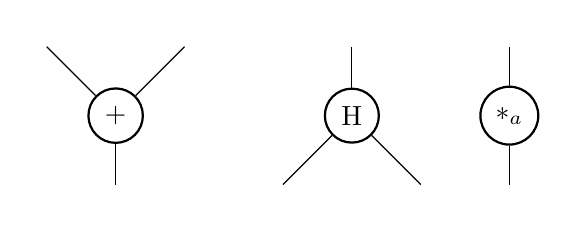
\begin{tikzpicture}
      \tikzstyle{node}=[circle,thick,draw=black,minimum size=4mm]
      
      \begin{scope}
        \node(in1){};
        \node(nop1)[right of=in1]{};
        \node(in2)[right of=nop1]{};
        \node(nop2)[right of=in2]{};
        \node(in3)[right of=nop2]{};
        \node(nop3)[right of=in3]{};
        \node(in4)[right of=nop3]{};
        
        \node[node](plus)[below of=nop1]{$+$}
        edge(in1)
        edge(in2);
        \node(nop)[below of=nop2]{};
        \node[node](hub)[below of=in3]{H}
        edge(in3);
        \node[node](times)[below of=in4]{$*_a$}
        edge(in4);
        
        \node(out1)[below of=plus]{}
        edge(plus);
        \node(nop5)[right of=out1]{};
        \node(out2)[below of=nop]{}
        edge(hub);
        \node(nop6)[below of=hub]{};
        \node(out3)[right of=nop6]{}
        edge(hub);
        \node(out4)[below of=times]{}
        edge(times);
      \end{scope}
    \end{tikzpicture}
  \end{center}
\end{frame}

%%

\begin{frame}
  \frametitle{Arithmetic circuits}

  \begin{columns}
    \begin{column}{0.6\textwidth}
      \centering
      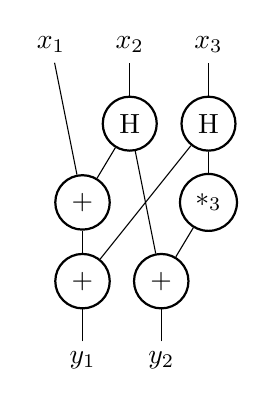
\begin{tikzpicture}
        \tikzstyle{node}=[circle,thick,draw=black,minimum size=4mm]
        
        \begin{scope}
          \node(x1){$x_1$};
          \node(x2)[right of=x1]{$x_2$};
          \node(x3)[right of=x2]{$x_3$};
          
          \node[node](d1)[below of=x2]{H}
          edge(x2);
          \node[node](d2)[below of=x3]{H}
          edge(x3);
          
          \node[node](p1)[below of=d1,xshift=-6mm]{$+$}
          edge(x1)
          edge(d1);
          \node[node](m1)[below of=d2]{$*_3$}
          edge(d2);
          
          \node[node](p2)[below of=p1]{$+$}
          edge(p1)
          edge(d2);
          \node[node](p3)[right of=p2]{$+$}
          edge(d1)
          edge(m1);
          
          \node(y1)[below of=p2]{$y_1$}
          edge(p2);
          \node(y2)[below of=p3]{$y_2$}
          edge(p3);
        \end{scope}
      \end{tikzpicture}
    \end{column}
    \begin{column}{0.4\textwidth}
      \begin{align*}
        y_1 &= x_1 + x_2 + x_3\\
        y_2 &= x_2 + 3x_3
      \end{align*}
      
      \Large
      \begin{gather*}
        \begin{pmatrix}
          1 & 1 & 1\\
          0 & 1 & 3
        \end{pmatrix}
      \end{gather*}
    \end{column}
  \end{columns}
\end{frame}

%%

\begin{frame}
  \frametitle{Transposition of an arithmetic circuit}

  \begin{columns}
    \begin{column}{0.6\textwidth}
      \centering
      \begin{tikzpicture}
        \tikzstyle{node}=[circle,thick,draw=black,minimum size=4mm]
        
        \begin{scope}
          \node(x1){$x_1$};
          \node(x2)[right of=x1]{$x_2$};
          \node(x3)[right of=x2]{$x_3$};
          
          \node[node](d1)[below of=x2]{H}
          edge(x2);
          \node[node](d2)[below of=x3]{H}
          edge(x3);
            
          \node[node](p1)[below of=d1,xshift=-6mm]{$+$}
          edge(x1)
          edge(d1);
          \node[node](m1)[below of=d2]{$*_3$}
          edge(d2);
          
          \node[node](p2)[below of=p1]{$+$}
          edge(p1)
          edge(d2);
          \node[node](p3)[right of=p2]{$+$}
          edge(d1)
          edge(m1);
          
          \node(y1)[below of=p2]{$y_1$}
          edge(p2);
          \node(y2)[below of=p3]{$y_2$}
          edge(p3);
        \end{scope}
        
        \begin{scope}[xshift=3.2cm, yshift=-0.23\textheight]
          \node(x){\Huge $\leftrightarrow$};
        \end{scope}
        
        \begin{scope}[xshift=4cm, yshift=-0.425\textheight]
          \node(x1){$x_1'$};
          \node(x2)[right of=x1]{$x_2'$};
          \node(x3)[right of=x2]{$x_3'$};
          
          \node[node](d1)[above of=x2]{\alt<2>{$+$}{H}}
          edge(x2);
          \node[node](d2)[above of=x3]{\alt<2>{$+$}{H}}
          edge(x3);
          
          \node[node](p1)[above of=d1,xshift=-5mm]{\alt<2>{H}{$+$}}
          edge(x1)
          edge(d1);
          \node[node](m1)[above of=d2]{$*_3$}
          edge(d2);
          
          \node[node](p2)[above of=p1]{\alt<2>{H}{$+$}}
          edge(p1)
          edge(d2);
          \node[node](p3)[right of=p2]{\alt<2>{H}{$+$}}
          edge(d1)
          edge(m1);
          
          \node(y1)[above of=p2]{$y_1'$}
          edge(p2);
          \node(y2)[above of=p3]{$y_2'$}
          edge(p3);
        \end{scope}
      \end{tikzpicture}
    \end{column}
    \begin{column}{0.4\textwidth}
      \begin{align*}
        y_1 &= x_1 + x_2 + x_3\\
        y_2 &= x_2 + 3x_3
      \end{align*}
      
      \Large
      \begin{gather*}
        \begin{pmatrix}
          1 & 1 & 1\\
          0 & 1 & 3
        \end{pmatrix}\\
        \updownarrow\\
        \begin{pmatrix}
          1 & 0\\
          1 & 1\\
          1 & 3\\
        \end{pmatrix}
      \end{gather*}
    \end{column}
  \end{columns}
\end{frame}

%%
%%

\begin{frame}
  \frametitle{Arithmetic Circuits: uniform vs. non-uniform}

  \begin{definition}[Circuit family]
    A \emph{circuit family} is a family $(C_0,C_1,\ldots)$ of circuits
    indexed by $\N$ such that $C_n$ has $n$ inputs.
  \end{definition}
  
  \begin{itemize}
  \item \alert{Any Turing-undecidable problem has a trivial
      \emph{polynomial-size} circuit family deciding it.}
  \end{itemize}

  \begin{definition}[Uniform circuit family]
    A circuit family $(C_0,C_1,\ldots)$ is said to be \emph{uniform}
    if there is a $\log n$-space bounded touring machine which on
    input $1^n$ outputs a representation of $C_n$.
  \end{definition}

  \begin{itemize}
  \item We will extend the definition to allow families to be indexed
    by any (countable) set $\mathcal{P}$, called the \emph{parameter
      space}.
  \end{itemize}
\end{frame}

%%

\begin{frame}[fragile]
  \frametitle{From non-uniform to uniform circuits?}
  
  {\large
    \begin{itemize}
    \item The transposition theorem easily generalises to non-uniform
      circuits.
    \item It can even be directly applied to computer programs (under
      certain hypotheses).
    \end{itemize}}

    \begin{columns}

    \begin{column}{0.5\textwidth}
      \begin{center}
        \begin{minipage}{0.7\textwidth}
\begin{semiverbatim}
  for i = 0 to n-2 do
    a[i+1] = a[i] + a[i+1]
    a[i] = 0
  end for
\end{semiverbatim}
        \end{minipage}
      \end{center}
    \end{column}

    \begin{column}{0.5\textwidth}

      \begin{equation*}
        \begin{pmatrix}
          0 & \hdotsfor{3} & 0\\
          \vdots  &  &\vdots&& \vdots \\
          0 & \hdotsfor{3} & 0\\
          1 & \hdotsfor{3} & 1
        \end{pmatrix}
      \end{equation*}

    \end{column}
  \end{columns}


\end{frame}

%%

\begin{frame}[fragile]
  \frametitle{From non-uniform to uniform circuits?}

  \begin{columns}
    \begin{column}{0.5\textwidth}
      \begin{center}
        \begin{minipage}{0.7\textwidth}
\begin{semiverbatim}
  a[1] = a[0] + a[1]
  a[0] = 0
  a[2] = a[1] + a[2]
  a[1] = 0
  ...
  a[n-1] = a[n-2] + a[n-1]
  a[n-2] = 0
\end{semiverbatim}
        \end{minipage}
      \end{center}
    \end{column}

    \begin{column}{0.5\textwidth}
      \begin{center}
        \begin{minipage}{0.7\textwidth}
\begin{semiverbatim}
  a[n-2] = 0
  a[n-2] = a[n-2] + a[n-1]
  ...
  a[1] = 0
  a[1] = a[1] + a[2]
  a[0] = 0
  a[0] = a[0] + a[1]
\end{semiverbatim}
        \end{minipage}
      \end{center}
    \end{column}
    \end{columns}
  
  \vfill

  \begin{columns}

    \begin{column}{0.5\textwidth}
      \begin{center}
        \begin{minipage}{0.7\textwidth}
\begin{semiverbatim}
  for i = n-2 to 0 do
    a[i] = 0
    a[i] = a[i] + a[i+1]
  end for
\end{semiverbatim}
        \end{minipage}
      \end{center}
    \end{column}

    \begin{column}{0.5\textwidth}

      \begin{equation*}
        \begin{pmatrix}
          0 & \hdotsfor{3} & 0\\
          \vdots  &  &\vdots&& \vdots \\
          0 & \hdotsfor{3} & 0\\
          1 & \hdotsfor{3} & 1
        \end{pmatrix}
      \end{equation*}

    \end{column}
  \end{columns}
\end{frame}

%%
%%

\section{Motivations}

\begin{frame}
  \frametitle{Minimal polynomials \cite{Sho95}}
  
  \vspace{-1ex}

  \begin{block}{Linear recurring sequences}
    An algebraic element $\sigma\in\LK=\K[X]/f(X)$, the $\sigma^i$'s
    satisfy a linear recurrence
    \[ \sigma^n = c_{n-1} \sigma^{n-1} + \cdots + c_1\sigma + c_0\]

    Let $\ell\in\LK^\ast$ a linear form, then
    \[ \ell(\sigma^n) = c_{n-1} \ell(\sigma^{n-1}) + \cdots +
    c_1\ell(\sigma) + c_0\ell(1)\]
  \end{block}

  \vspace{-1ex}

  \begin{block}{Power projection}
    Given $\ell$ and $\sigma$, the power projection problem asks to
    compute
    \[\ell(1), \ell(\sigma), \ell(\sigma^2), \ldots, \ell(\sigma^{n-1})\]
    For fixed $\sigma$, it is a $\K$-linear map, its transpose is the map
    \[g\mapsto g(\sigma) \bmod f\]
    hence its transpose problem is \emph{modular composition}.
  \end{block}
\end{frame}

%%

\begin{frame}
  \frametitle{Applications}

  \begin{block}{Uses and generalisations of power projection}
    \begin{itemize}
    \item Minimal polynomials in towers of extension fields \cite{Sho95}.
    \item Change of order in triangular sets.
    \item Change of order in Artin-Schreier towers \cite{DFS09},
      application to isogeny computation.
    \end{itemize}
  \end{block}

  \begin{block}{Other applications}
    \begin{itemize}
    \item Generation of irreducible polynomials.
    \item Complexity bounds on evaluation/interpolation.
    \item Reverse mode in automatic differentiation.
    \end{itemize}
  \end{block}
\end{frame}

%%

\begin{frame}
  \frametitle{Other motivations}

  \begin{quote}
    ``The author has not been able to find an example of a linear
    operator that is easy to apply but whose transpose is difficult to
    apply.''
  \end{quote}
  \hfill\cite{Wie86}
  
  \begin{quote}
    ``The transposition principle is very useful for proving the
    existence of algorithms, but actually coming up with an explicit,
    practical algorithm requires a bit more effort.''
  \end{quote}
  \hfill\cite{Sho95}

  \begin{quote}
    ``We offer no other proof of correctness other than the validity
    of this transformation technique (and the fact that it does indeed
    work in practice).''
  \end{quote}
  \hfill\cite{Sho95}

  \begin{quote}
    ``Oulala ! Vous avez encore utilisé votre magie noire !''
  \end{quote}
  \hfill François Morain, personal communication
\end{frame}

%%

\begin{frame}[fragile]
  \tiny
  \frametitle{Other motivations}

  \begin{columns}
    \begin{column}{0.5\textwidth}
      \begin{center}
        \begin{minipage}{\textwidth}
\begin{verbatim}
void reduc_doit(GF2X& A0, GF2X& A1, const GF2X& A,
	long init, long d, bool plusone){
  if (d <= 2){
    A0 = GF2X(0, coeff(A,init));
    A1 = GF2X(0, coeff(A,init+1));
    return;
  }
   
  long dp = d/2;
  GF2X A10, A11;

  reduc_doit(A0, A1, A, init, dp, plusone);
  reduc_doit(A10, A11, A, init+dp, dp, plusone);
 
  ShiftAdd(A0, A11, 1);
  if (plusone) A0 += A11;
  A1 += A10 + A11;

  long i = 1;
  bool even = true;
  while (2*i != d){
    ShiftAdd(A0, A10, i);
    ShiftAdd(A1, A11, i);
    i = 2*i;
    even = !even;
  }
  
  if (plusone && !even) {
    A0 += A10;
    A1 += A11;
  }
}
\end{verbatim}
        \end{minipage}
      \end{center}
    \end{column}

    \begin{column}{0.5\textwidth}
      \begin{center}
        \begin{minipage}{\textwidth}
\begin{verbatim}
void treduc_doit(GF2X& A, const GF2X& A0, const GF2X& A1, long d,
	bool plusone){
  if (d <= 2){
    SetCoeff(A, 0, coeff(A0, 0));
    SetCoeff(A, 1, coeff(A1, 0));
    return;
  }
   
  long dp = d/2;
  long hdp = dp/2;

  GF2X A00, A01, A10, A11;
  A00 = trunc(A0, hdp);
  A01 = trunc(A1, hdp);

  A10 = A01;
  if (plusone) A11 = A00;
  else A11 = 0;
  A11 += A01 + RightShift(trunc(A0, hdp+1), 1);
  long i = 1;
  bool even = true;
  while (2*i != d){
    A10 += RightShift(trunc(A0, hdp+i), i);
    A11 += RightShift(trunc(A1, hdp+i), i);
    i = 2*i;
    even = !even;
  }
  
  if (plusone && !even) {
    A10 += trunc(A0, hdp);
    A11 += trunc(A1, hdp);
  }
  
  GF2X B0, B1;
  treduc_doit(B0, A00, A01, dp, plusone);
  treduc_doit(B1, A10, A11, dp, plusone);
  A = B0 + LeftShift(B1,dp);
}
\end{verbatim}
        \end{minipage}
      \end{center}
    \end{column}
    \end{columns}
\end{frame}

%%

\begin{frame}
  \frametitle{Other motivations}

  \begin{quote}
    In developing transposed code for our ISSAC '09 paper, a very
    tricky mistake slowed down performances by more than a constant
    factor. The bug was so subtle that in the first place we didn't
    even think there was one; a machine wouldn't have made the
    mistake.
  \end{quote}
  \hfill

  \begin{quote}
    A striking similarity with reversible computation and quantum
    circuits.
  \end{quote}
  \hfill

  \begin{quote}
    A never (so I thought) enough studied relationship with automatic
    differentiation.
  \end{quote}
  \hfill

  \begin{quote}
    A long history of re-discoveries and many different formulations.
  \end{quote}
\end{frame}

%%

\begin{frame}
  \frametitle{History}

  \begin{block}{History}
    \begin{itemize}
    \item Originally discovered in \emph{electrical network theory}
      \cite{Bor56} (only works for $\C$);
    \item \cite{BCS} attribute the discovery to Tellegen, Bordewijk's
      director, but this is debated;
    \item Graph-theoretic approach by Fettweis (1971) for
      \emph{digital filters};
    \item \cite{Fid73} and \cite{HoMu73}: transposition of
      \emph{bilinear chains}, the most complete formulation
      (non-commutative rings);
    \item Special case of \emph{automatic differentiation}
      \cite{BS83};
    \item In \emph{computer algebra}, popularized by Shoup, von zur
      Gathen, Kaltofen,\dots
    \item \cite{BLS03} improve algorithms for polynomial evaluation
      and solve an open question on space complexity.
    \end{itemize}
  \end{block}
\end{frame}

%%
%%

\section{Circuit emulation}

\begin{frame}
  \frametitle{Multilinearity}

  \begin{center}
    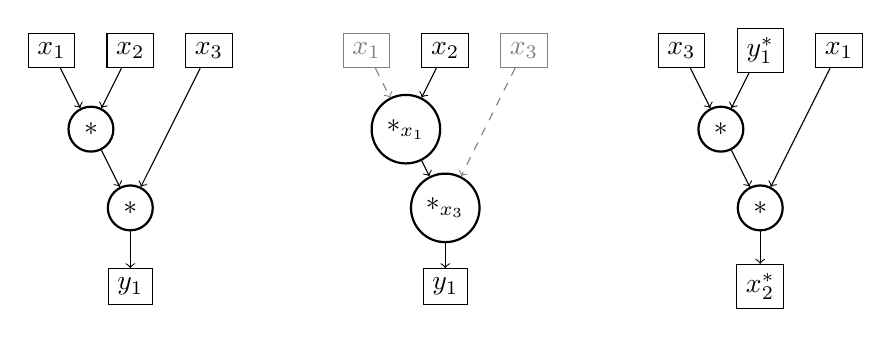
\begin{tikzpicture}
      \tikzstyle{node}=[circle,thick,draw=black,minimum size=4mm]
      \tikzstyle{arg}=[rectangle,thin,draw=black,minimum size=4mm]
      \tikzstyle{nodeg}=[circle,thick,draw=gray,minimum size=4mm]
      \tikzstyle{argg}=[rectangle,thin,draw=gray,minimum size=4mm]
      
      \begin{scope}
        \node[arg](in1){$x_1$};
        \node[arg,right of=in1](in2){$x_2$};
        \node[arg,right of=in2](in3){$x_3$};
        \node[node,below of=in1,xshift=5mm](times1){$*$};
        \node[node,below of=times1,xshift=5mm](times2){$*$};
        \node[arg,below of=times2](out){$y_1$};
        
        \path[->]
        (in1) edge (times1)
        (in2) edge (times1)
        (times1) edge (times2)
        (in3) edge (times2)
        (times2) edge (out);
      \end{scope}
      
      \begin{scope}[xshift=4cm]
        \node[argg](in1){\color{gray}{$x_1$}};
        \node[arg,right of=in1](in2){$x_2$};
        \node[argg,right of=in2](in3){\color{gray}{$x_3$}};
        \node[node,below of=in1,xshift=5mm](times1){$*_{x_1}$};
        \node[node,below of=times1,xshift=5mm](times2){$*_{x_3}$};
        \node[arg,below of=times2](out){$y_1$};
        
        \path[->]
        (in2) edge (times1)
        (times1) edge (times2)
        (times2) edge (out);
        
        \path[->,draw=gray,dashed]
        (in1) edge (times1)
        (in3) edge (times2);
      \end{scope}
      
      \begin{scope}[xshift=8cm]
        \node[arg](in1){$x_3$};
        \node[arg,right of=in1](in2){$y_1^\ast$};
        \node[arg,right of=in2](in3){$x_1$};
        \node[node,below of=in1,xshift=5mm](times1){$*$};
        \node[node,below of=times1,xshift=5mm](times2){$*$};
        \node[arg,below of=times2](out){$x_2^\ast$};

        \path[->]
        (in2) edge (times1)
        (times1) edge (times2)
        (times2) edge (out)
        (in3) edge (times2)
        (in1) edge (times1);
      \end{scope}
    \end{tikzpicture}  
  \end{center}

  \begin{itemize}
  \item Almost anytime we want to transpose, we end-up
    \emph{linearising} a circuit with multiplication nodes.
  \item Other constructs such as \texttt{if} statements and
    \texttt{for} loops need to be linearised too.
  \end{itemize}
\end{frame}

%%

\begin{frame}[fragile]
  \frametitle{Circuit emulation}

  \begin{lstlisting}
    karatsuba [] y n = []

    karatsuba x [] n = []

    karatsuba x y n =
      if n <= 0
      then []
      else if n == 1 
           then [(x!!0) * (y!!0)]
           else 
             let h = n / 2 in
             let (a0, a1) = split x h in
             let (b0, b1) = split y h in
             let x0 = karatsuba a0 b0 h in
             let x2 = karatsuba a1 b1 (n-h) in
             let xx1 = karatsuba (a1 + a0) (b1 + b0) (n-h) in
             let x1 = xx1 + ((x0 + x2) * (- one)) in
             (shift x2 n) + (shift x1 h) + x0
  \end{lstlisting}
\end{frame}

%%

\begin{frame}[fragile]
  \frametitle{Circuit emulation}

  \begin{lstlisting}
    karatsuba x n =
      if n <= 0
      then []
      else if n == 1 
           then \y -> [(x!!0) * (y!!0)]
           else 
             let h = n / 2 in
             let (a0, a1) = split x h in
             let x0 = karatsuba a0 h in
             let x2 = karatsuba a1 (n-h) in
             let xx1 = karatsuba (a1 + a0) (n-h) in
             let sp = \y -> split y h in
             let sh1 = \y -> shift y n in
             let sh2 = \y -> shift y h in

             \y -> .... 
  \end{lstlisting}
\end{frame}

%%

\begin{frame}[fragile]
  \frametitle{Circuit emulation}

  \begin{lstlisting}
    let h = n / 2 in
    let (a0, a1) = split x h in
    let x0 = karatsuba a0 h in
    let x2 = karatsuba a1 (n-h) in
    let xx1 = karatsuba (a1 + a0) (n-h) in
    let sp = Circuit(\y -> split y h) in
    let sh1 = Circuit(\y -> shift y n) in
    let sh2 = Circuit(\y -> shift y h) in
    
    proc y -> do
      (y0, y1) <- sp -< y 
      s0 <- x0 -< y0
      s2 <- x2 -< y1
      ss1 <- (id <+> id).xx1 -< (y0, y1)
      s1 <- id <+> ((id <+> id) <*> (- one)) -< (ss1, (s0, s2))
      z <- sh1 <+> sh2 <+> id -<  (s2, (s1, s0))
      returnA -< z
  \end{lstlisting}
\end{frame}

%%
%%

\section{Automatic differentiation}

\begin{frame}
  \frametitle{Automatic differentiation of circuits \cite{BS83}}

  \begin{center}
    Transformation technique on circuits $R^n\ra R^m$:\\
    node $\mapsto$ its Jacobian at point $x$\\
    (we are overly vulgarising, there's more than that in reality)
  \end{center}

  \begin{center}
    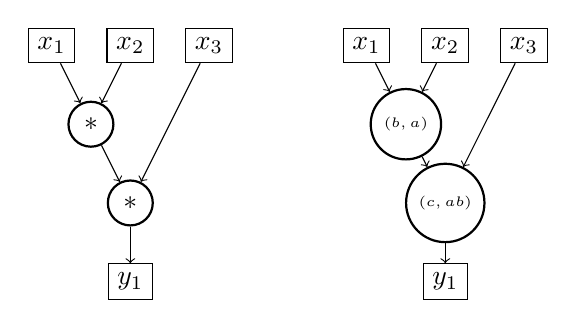
\begin{tikzpicture}
      \tikzstyle{node}=[circle,thick,draw=black,minimum size=4mm]
      \tikzstyle{arg}=[rectangle,thin,draw=black,minimum size=4mm]
      
      \begin{scope}
        \node[arg](in1){$x_1$};
        \node[arg,right of=in1](in2){$x_2$};
        \node[arg,right of=in2](in3){$x_3$};
        \node[node,below of=in1,xshift=5mm](times1){$*$};
        \node[node,below of=times1,xshift=5mm](times2){$*$};
        \node[arg,below of=times2](out){$y_1$};
        
        \path[->]
        (in1) edge (times1)
        (in2) edge (times1)
        (times1) edge (times2)
        (in3) edge (times2)
        (times2) edge (out);
      \end{scope}

      \begin{scope}[xshift=4cm]
        \node[arg](in1){$x_1$};
        \node[arg,right of=in1](in2){$x_2$};
        \node[arg,right of=in2](in3){$x_3$};
        \node[node,below of=in1,xshift=5mm](times1){\tiny$(b,a)$};
        \node[node,below of=times1,xshift=5mm](times2){\tiny$(c,ab)$};
        \node[arg,below of=times2](out){$y_1$};
        
        \path[->]
        (in1) edge (times1)
        (in2) edge (times1)
        (times1) edge (times2)
        (in3) edge (times2)
        (times2) edge (out);
      \end{scope}
    \end{tikzpicture}
  \end{center}

  \begin{itemize}
  \item By the chain rule, the result computes the Jacobian of the
    circuit.
  \item Evaluating on a vector gives a directional derivative
  \item $n$ directional derivatives yield the whole Jacobian.
  \end{itemize}
\end{frame}

%%

\begin{frame}
  \frametitle{Reverse mode}

  \begin{center}
    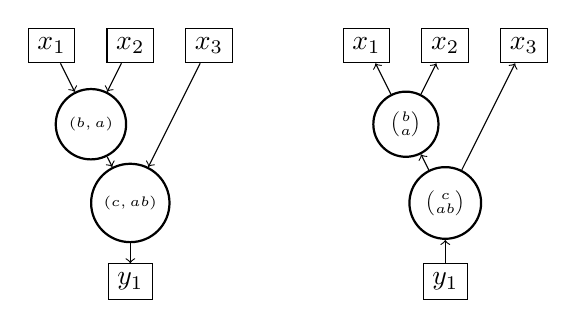
\begin{tikzpicture}
      \tikzstyle{node}=[circle,thick,draw=black,minimum size=4mm]
      \tikzstyle{arg}=[rectangle,thin,draw=black,minimum size=4mm]
      
      \begin{scope}
        \node[arg](in1){$x_1$};
        \node[arg,right of=in1](in2){$x_2$};
        \node[arg,right of=in2](in3){$x_3$};
        \node[node,below of=in1,xshift=5mm](times1){\tiny$(b,a)$};
        \node[node,below of=times1,xshift=5mm](times2){\tiny$(c,ab)$};
        \node[arg,below of=times2](out){$y_1$};
        
        \path[->]
        (in1) edge (times1)
        (in2) edge (times1)
        (times1) edge (times2)
        (in3) edge (times2)
        (times2) edge (out);
      \end{scope}

      \begin{scope}[xshift=4cm]
        \node[arg](in1){$x_1$};
        \node[arg,right of=in1](in2){$x_2$};
        \node[arg,right of=in2](in3){$x_3$};
        \node[node,below of=in1,xshift=5mm](times1){\tiny$\binom{b}{a}$};
        \node[node,below of=times1,xshift=5mm](times2){\tiny$\binom{c}{ab}$};
        \node[arg,below of=times2](out){$y_1$};
        
        \path[->]
        (times1) edge (in1) 
        (times1) edge (in2) 
        (times2) edge (times1) 
        (times2) edge (in3) 
        (out) edge (times2);
      \end{scope}
    \end{tikzpicture}
  \end{center}

  \begin{block}{Reverse mode}
    \begin{itemize}
    \item After transposition, $m$ directional derivatives suffice to
      compute the Jacobian,
    \item In particular, for a map $R^n\ra R$, only one evaluation is
      needed to compute the gradient.
    \end{itemize}
  \end{block}
\end{frame}

%%

\begin{frame}
  \frametitle{Transposing with AD tools}

  \begin{center}
    AD tools work on straight line programs, they implicitly implement
    transposition in reverse mode
  \end{center}

  \begin{block}{But !}
    \begin{itemize}
    \item They cost too much in space, because they have to precompute
      the circuit,
    \item Iterative statements can cause memory swell,
    \item They are only useful in the case $R^n\ra R$,
    \item They can't handle multilinearity,
    \item They can't handle recursive calls (as far as I have seen).
    \end{itemize}
  \end{block}
\end{frame}
%%
%%

\section{Linearity inference}

\begin{frame}
  \frametitle{Multilinearity}

  \begin{center}
    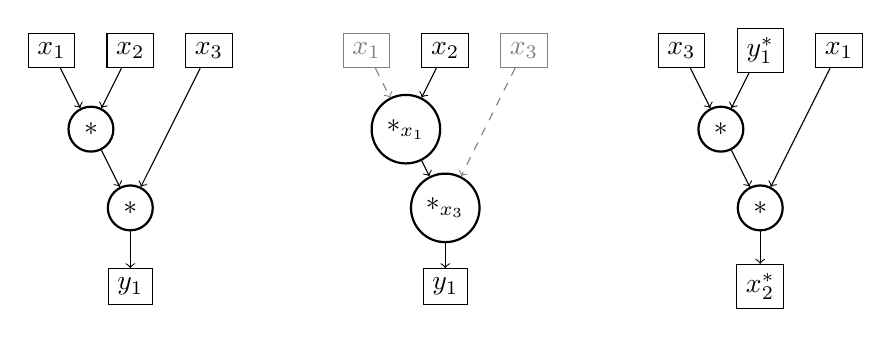
\begin{tikzpicture}
      \tikzstyle{node}=[circle,thick,draw=black,minimum size=4mm]
      \tikzstyle{arg}=[rectangle,thin,draw=black,minimum size=4mm]
      \tikzstyle{nodeg}=[circle,thick,draw=gray,minimum size=4mm]
      \tikzstyle{argg}=[rectangle,thin,draw=gray,minimum size=4mm]
      
      \begin{scope}
        \node[arg](in1){$x_1$};
        \node[arg,right of=in1](in2){$x_2$};
        \node[arg,right of=in2](in3){$x_3$};
        \node[node,below of=in1,xshift=5mm](times1){$*$};
        \node[node,below of=times1,xshift=5mm](times2){$*$};
        \node[arg,below of=times2](out){$y_1$};
        
        \path[->]
        (in1) edge (times1)
        (in2) edge (times1)
        (times1) edge (times2)
        (in3) edge (times2)
        (times2) edge (out);
      \end{scope}
      
      \begin{scope}[xshift=4cm]
        \node[argg](in1){\color{gray}{$x_1$}};
        \node[arg,right of=in1](in2){$x_2$};
        \node[argg,right of=in2](in3){\color{gray}{$x_3$}};
        \node[node,below of=in1,xshift=5mm](times1){$*_{x_1}$};
        \node[node,below of=times1,xshift=5mm](times2){$*_{x_3}$};
        \node[arg,below of=times2](out){$y_1$};
        
        \path[->]
        (in2) edge (times1)
        (times1) edge (times2)
        (times2) edge (out);
        
        \path[->,draw=gray,dashed]
        (in1) edge (times1)
        (in3) edge (times2);
      \end{scope}
      
      \begin{scope}[xshift=8cm]
        \node[arg](in1){$x_3$};
        \node[arg,right of=in1](in2){$y_1^\ast$};
        \node[arg,right of=in2](in3){$x_1$};
        \node[node,below of=in1,xshift=5mm](times1){$*$};
        \node[node,below of=times1,xshift=5mm](times2){$*$};
        \node[arg,below of=times2](out){$x_2^\ast$};

        \path[->]
        (in2) edge (times1)
        (times1) edge (times2)
        (times2) edge (out)
        (in3) edge (times2)
        (in1) edge (times1);
      \end{scope}
    \end{tikzpicture}  
  \end{center}

  \begin{itemize}
  \item Can we automatically deduce any possible linearisation of a
    program?
  \item Type inference systems can help us
  \end{itemize}
\end{frame}

%%

\begin{frame}[fragile]
  \frametitle{Linearity inference}

  \begin{center}
    Suppose given a type \lstinline{R} implementing a ring. We want to
    define types \lstinline{L} (for \emph{linear}) and \lstinline{S}
    (for scalar) such that the following equations hold
  \end{center}

  \begin{lstlisting}
    plus :: L -> L -> L
    plus :: S -> S -> S
    times :: L -> S -> L
    times :: S -> S -> S
    zeroR :: L
    zeroR :: S
    oneR :: S
  \end{lstlisting}
\end{frame}  

\begin{frame}[fragile]
  \frametitle{Linearity inference}
  
  \begin{center}
    Here's the solution    
  \end{center}

  \begin{lstlisting}
    data L = L R
    data S = S R
    
    class Ring r where
      zero :: r
      (<+>) :: r -> r -> r
      neg :: r -> r
      (<*>) :: r -> S -> r

    one = S oneR
    (S a) == (S b) = a == b
  \end{lstlisting}

  \begin{center}
    Let's check it in a shell
  \end{center}
\end{frame}

%%
%%

\section{Automatic transposition}

\lstset{language=python}

\begin{frame}[fragile]
  \frametitle{The Transposable Algebraic Language}

  \begin{block}{Algebraic types}
    \begin{itemize}
    \item \textbf{Prototypes}: {\tt Ring}, {\tt Module}, (optionally
      {\tt Algebra}, \dots)
    \item Declaring an algebraic type:
\begin{lstlisting}
  type Ring R
  type Module(R) M
\end{lstlisting}
    \end{itemize}
  \end{block}

  \begin{block}{Declaring a function}
\begin{lstlisting}
  fun (linear M A, const m)f(linear M Z, const M z, const n):
\end{lstlisting}
  \end{block}

  \begin{block}{Other constructs}
    \begin{itemize}
    \item Standard types ({\tt int}, {\tt bool}, \ldots)
    \item {\tt if}, {\tt match}, recursion, {\tt let} binding,
    \item Algebraic operators $+$, $\times$, projection/injection
      \verb|a[n]|.
    \end{itemize}
  \end{block}
\end{frame}

%%

\begin{frame}[fragile]
  \frametitle{Automatic transposition: the general algorithm}

\begin{lstlisting}
  fun (linear R res)scalar(linear M a, const n):
    if n = 0:
      res = 0
    else:
      res = a[n] + scalar(a, n-1)
\end{lstlisting}

  \begin{block}{The algortithm}
    \begin{itemize}
    \item First run the algorithm in the normal direction to compute
      all the {\tt const} values,
    \item then run the algorithm backwards transposing each instruction.
    \end{itemize}
  \end{block}

\begin{lstlisting}
  fun (linear M a)scalar^T(linear R res, const n):
    if n = 0:
      nop
    else:
      a[n] = res
      a += scalar^T(res, n-1)
\end{lstlisting}
\end{frame}

%%

\begin{frame}
  \frametitle{Scalar prediction and tail recursion}

  \begin{itemize}
  \item Permuting the order of the instructions may break tail/head
    recursion,
  \item this implies loss of efficiency,
  \item equivalently, in {\tt for} loops we have to precompute all the
    {\tt const} values of the loop,
  \item \alert{this seems to increase the space requirements of the
      algorithm}, but does not affect the number of arithmetic operations.
  \end{itemize}
\end{frame}

%%

\begin{frame}[fragile]
  \frametitle{Scalar prediction and tail recursion}

  \begin{columns}
    \begin{column}{0.5\textwidth}
\begin{lstlisting}
fun (R a, R b)f(R c, R d):
  if d > 0:
    x, y = f(c, d - 1)
    a, b = x * y, y + 1
  else:
    a, b = c, d
\end{lstlisting}
    \end{column}
    \begin{column}{0.5\textwidth}
\begin{lstlisting}
fun (R c, R b)fT(R a, R d):
  # Forward sweep
  if (d > 0):
    _, y = f(a, d - 1)
    b = y + 1
  else:
    b = d
    
  # Reverse sweep
  if (d > 0):
    x = a * y
    c, y = fT(x, d - 1)
  else:
    c = a
\end{lstlisting}      
    \end{column}
  \end{columns}
\end{frame}

%%
%%

\section{\tALpy}

\begin{frame}
  \frametitle{A Python implementation of TransAL}

  \begin{center}
    \Large
    \url{http://transalpyne.gforge.inria.fr/}
  \end{center}

  \begin{itemize}
  \item Compiler/interpreter written in python,
  \item python-like syntax,
  \item automated constness inference,
  \item smart handling of array sizes,
  \item will compile to other languages (Haskell? OCaml?).
  \end{itemize}
\end{frame}

%%

\begin{frame}[fragile]
  \frametitle{Karatsuba in \tALpy}

\begin{lstlisting}
def (M c)karatsuba(M a, M b, n):
  if n == 1:
    tmp = M.zero()
    tmp[0] += a[0]*b[0]
    c = tmp
  elif n > 1:
    a0, a1 = split(a, n/2, n)
    b0, b1 = split(b, n/2, n)
    x0 = karatsuba(a0, b0, n/2)
    x2 = karatsuba(a1, b1, n - n/2)
    x1 = karatsuba((a1 + a0), (b1 + b0), n - n/2) - x0 - x2
    c = shift(x2, n, n+1) + shift(x1, n/2, n+1) + x0
\end{lstlisting}
\end{frame}

%%

\begin{frame}[fragile]
  \frametitle{Karatsuba in \tALpy}

  \lstset{basicstyle=\ttfamily\footnotesize}
\begin{lstlisting}
(M b)karatsubaT(M a, M c, n)
  # Forward sweep
  if (n == 1):
    pass
  elif n > 1:
    a0, a1 = split(a, n / 2, n)
  # Reverse sweep
  if (n == 1):
    tmp = c
    _transAL_tmp_0[0] += a[0] * tmp[0]
    b = _transAL_tmp_0
  elif n > 1:
    x2 = trans shift(c, n, n + 1)
    x1 = trans shift(c, n / 2, n + 1)
    x0 = c
    b1 = trans karatsuba(x1, a1 + a0, n - n / 2)
    b0 = b1
    x0 += - x1
    x2 += - x1
    b1 += trans karatsuba(x2, a1, n - n / 2)
    b0 += trans karatsuba(x0, a0, n / 2)
    b = trans split(b0, b1, n / 2, n)
\end{lstlisting}
\end{frame}

%%
%%

\begin{frame}
  \frametitle{Bibliography}

  \begin{thebibliography}{1}
    
  \bibitem[Baur, Strassen '83]{BS83}
    W.~Baur and V.Strassen.
    \newblock The complexity of computing partial derivatives.
    \newblock \emph{Theoretical Computer Science} 22, pp. 317--330, 1983.

  \bibitem[Bordewijk '56]{Bor56}
    J.~L.~Bordewijk.
    \newblock Inter-reciprocity applied to electrical networks
    \newblock \emph{Applied Scientific Research B: Electrophysics, Acoustics, Optics, Mathematical Methods} 6, pages 1--74, 1956.

  \bibitem[Bostan, Lercerf, Schost '03]{BLS03}A.~Bostan, G.~Lecerf \& E.~Schost,
    \newblock Tellegen's Principle into Practice.
    \newblock \emph{Proceedings of ISAAC 2003}.

  \bibitem[B\"urgisser, Clausen, Shokrollahi]{BCS}P.~Bürgisser, M.~Clausen \& M.~A.~Shokrollahi,
    \newblock \emph{Algebraic Complexity Theory}.
    \newblock Springer, 1997.

  \bibitem[D.F., Schost '09]{DFS09}
    L.~De~Feo and {\'E}.~Schost.
    \newblock Fast arithmetics in Artin-Schreier towers over finite fields. 
    \newblock In \emph{ISSAC'09}, pages 127--134. ACM, 2010.

  \end{thebibliography}
\end{frame}

\begin{frame}
  \frametitle{Bibliography}

  \begin{thebibliography}{1}
  
  \bibitem[Fiduccia '73]{Fid73}
    C.~M.~Fiduccia.
    \newblock \emph{On the algebraic complexity of matrix multiplication}
    \newblock PhD Thesis, Brown University, 1973.

  \bibitem[Hopcroft, Musinski '73]{HoMu73}
    J.~Hopcroft and J.~Musinski.
    \newblock Duality applied to the complexity of matrix multiplication
    and other bilinear forms.
    \newblock \emph{SIAM Journal on Computing}, vol. 2, pp. 159–173, 1973.

  \bibitem[Kaltofen '00]{Ka2k}
    E.~Kaltofen.
    \newblock Challenges of symbolic computation: my
    favorite open problems.
    \newblock \emph{Journal of Symbolic Computation}, 29(6):891--919, 2000.

  \bibitem[Shoup '95]{Sho95}
    V.~Shoup.
    \newblock A new polynomial factorization algorithm and its implementation.
    \newblock \emph{J. Symb. Comp.}, 20(4):363--397, 1995.
    
  \bibitem[Wiedemann '86]{Wie86}
    D.~H.~Wiedemann.
    \newblock Solving Sparse Linear Equations Over Finite Fields.
    \newblock \emph{IEEE Trans. Inf. Theory}, vol. IT-32:54--62, 1986.

  \end{thebibliography}
\end{frame}

\end{document}





%%% Local Variables: 
%%% mode:flyspell
%%% ispell-local-dictionary:"british"
%%% mode: TeX-PDF
%%% TeX-master: t
%%% End: 
%
% LocalWords:  Tellegen